\section{Theory Foundation}

\subsection{Webserver}
A web server is a software component that receives HTTP or HTTPS requests from clients and returns appropriate responses. It can deliver static resources, such as HTML, CSS, JavaScript, and images, or forward requests to an application server for further processing. Web servers can also support functions such as request routing, HTTPS termination, and reverse proxying, depending on their configuration.

\subsection{Transaction Script pattern}
Transaction script pattern organizes business logic by procedure where each procedure handles a single request from the presentation. Moodle mostly follow a transaction script approach. For example, if you open the Moodle forum page, the URL may be \textit{…/mod/forum/view.php?id=1234} in which the \textit{mod/forum/view.php} is the script that generates that page.

\subsection{SQL}
Structured Query Language is a standard, high-level, declarative language used to interact with relational database management systems (RDBMS). It allows users and applications to define database structures, retrieve and modify data, define views, specify access permissions and integrity constraints, and control transactions. As a non-procedural language, SQL specifies what data is required rather than how the database should process the request.

\subsection{ERD (Chen Notation ERD)}
The entity-relationship model represents the real world using entities, relationships, and their attributes. It can used as a basis for a unified view of data. An entity-relationship diagram is used to visualize this model. In this project, we will use the Chen notation ERD.

\begin{enumerate}
    \item \textbf{Entities:} A thing or an object in the real world with an independent existence, being distinguishable.
    \begin{figure}[H]
        \centering
        \begin{minipage}[t]{0.4\textwidth}
            \centering
            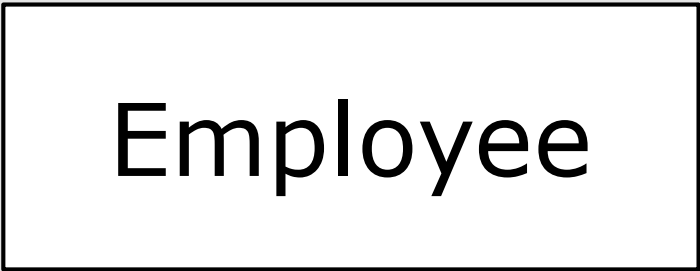
\includegraphics[width=\linewidth]{images/erd/entity.png}
            \caption{Entity Type}
            \label{fig:entity}
        \end{minipage}%
        \hspace{1cm}%
        \begin{minipage}[t]{0.4\textwidth}
            \centering
            
\includegraphics[width=\linewidth]{images/erd/weakentity.png}
            \caption{Weak Entity Type}
            \label{fig:entity-weak}
        \end{minipage}
    \end{figure}
    \item \textbf{Attributes:} A particular property that describes
an entity via a value.
    \begin{figure}[H]
        \centering
        \begin{minipage}[t]{0.4\textwidth}
            \centering
            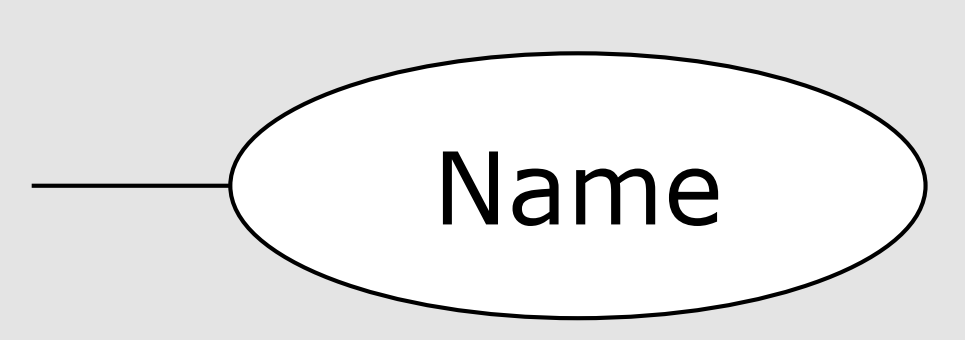
\includegraphics[width=\linewidth]{images/erd/attribute.png}
            \caption{Attribute}
            \label{fig:attribute}
        \end{minipage}%
        \hspace{1cm}%
        \begin{minipage}[t]{0.4\textwidth}
            \centering
            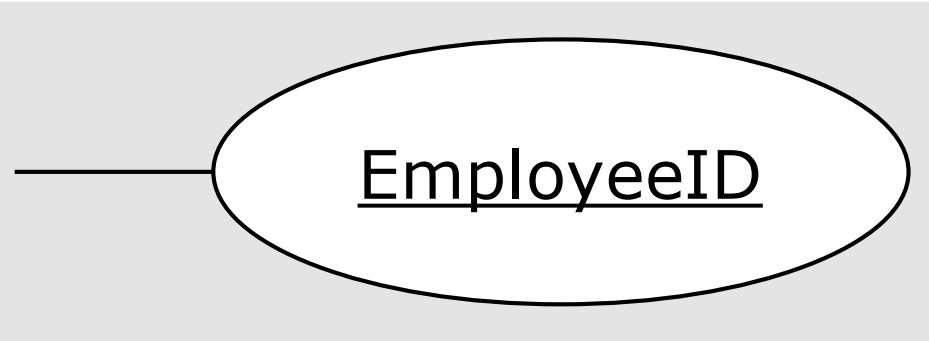
\includegraphics[width=\linewidth]{images/erd/keyattribute.png}
            \caption{Key Attribute}
            \label{fig:key-attribute}
        \end{minipage}
    \end{figure}
    \begin{figure}[H]
        \centering
        \begin{minipage}[t]{0.4\textwidth}
            \centering
            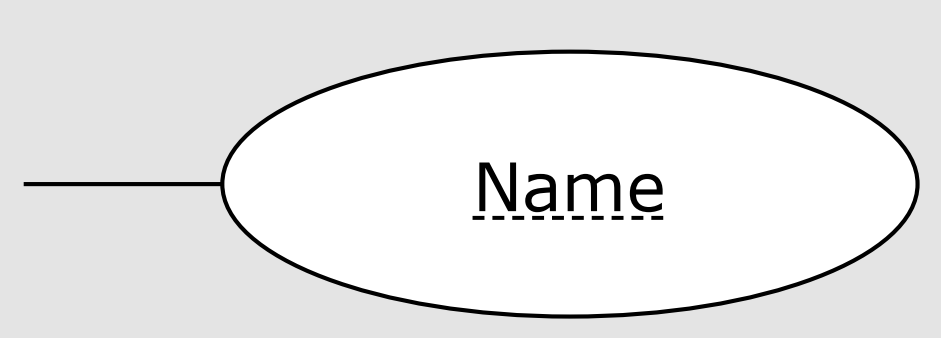
\includegraphics[width=\linewidth]{images/erd/partialattribute.png}
            \caption{Partial Key Attribute}
            \label{fig:partial-key-attribute}
        \end{minipage}%
        \hspace{1cm}%
        \begin{minipage}[t]{0.4\textwidth}
            \centering
            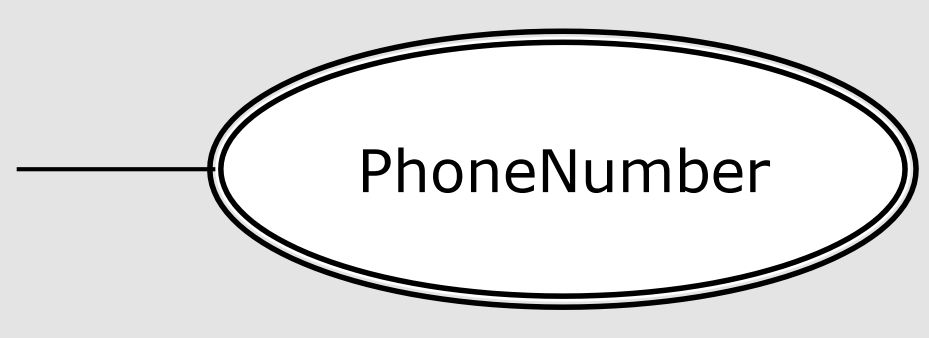
\includegraphics[width=\linewidth]{images/erd/multivaluedattribute.png}
            \caption{Multivalued Attribute}
            \label{fig:multivalued-attribute}
        \end{minipage}
    \end{figure}
    \begin{figure}[H]
        \centering
        \begin{minipage}[t]{0.4\textwidth}
            \centering
            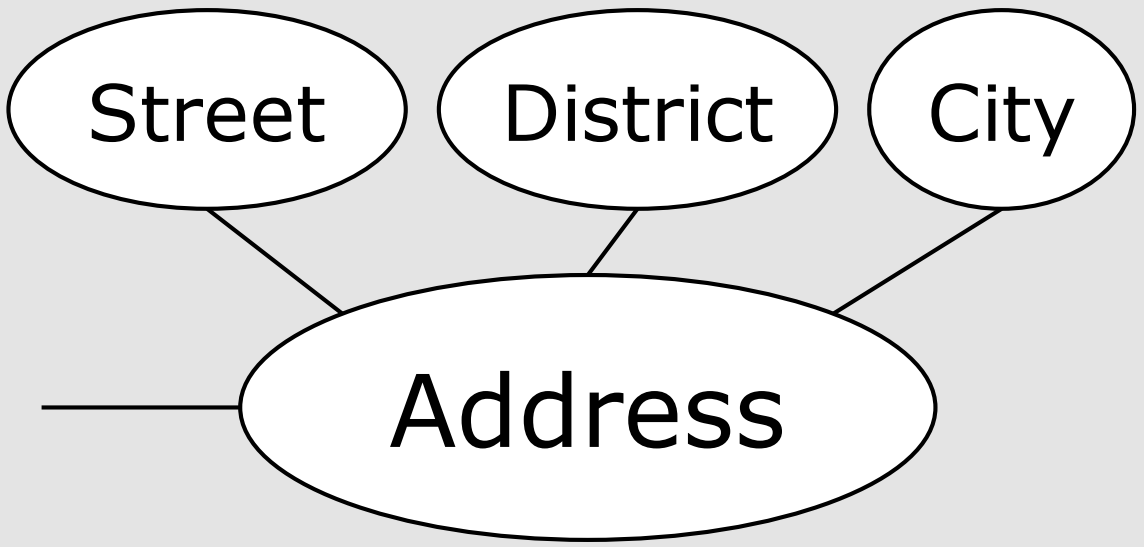
\includegraphics[width=\linewidth]{images/erd/compositeattribute.png}
            \caption{Composite Attribute}
            \label{fig:composite-attribute}
        \end{minipage}%
        \hspace{1cm}%
        \begin{minipage}[t]{0.4\textwidth}
            \centering
            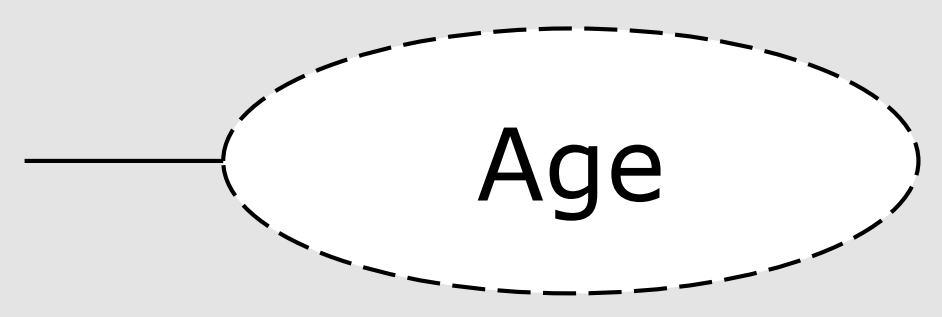
\includegraphics[width=\linewidth]{images/erd/deviredattribute.png}
            \caption{Devired Attribute}
            \label{fig:devired-attribute}
        \end{minipage}
    \end{figure}
    \item \textbf{Relationships:} A set of associations among entities.
    \begin{figure}[H]
        \centering
        \begin{minipage}[t]{0.4\textwidth}
            \centering
            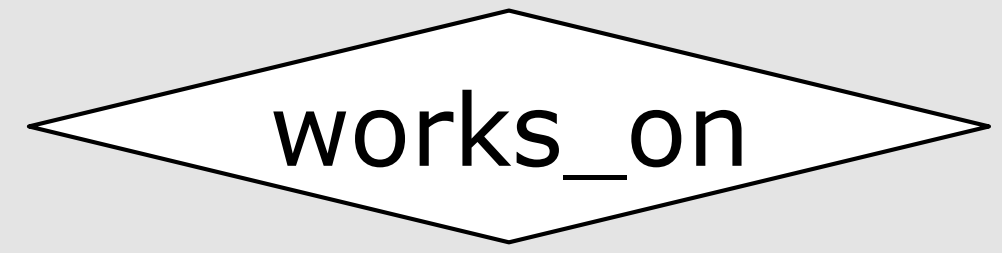
\includegraphics[width=\linewidth]{images/erd/relationship.png}
            \caption{Relationship Type}
            \label{fig:relationship}
        \end{minipage}%
        \hspace{1cm}%
        \begin{minipage}[t]{0.4\textwidth}
            \centering
            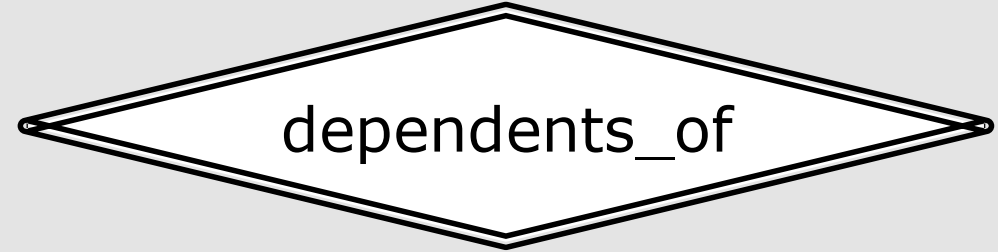
\includegraphics[width=\linewidth]{images/erd/weakrelationship.png}
            \caption{Relationship Type of Weak Entity Type}
            \label{fig:weak-relationship}
        \end{minipage}
    \end{figure}
    \item \textbf{Structural Constraints:} Limitations and rules on how entities participate in relationships, determining valid data configurations.
    \begin{itemize}
        \item \textbf{Single line:} Partial participation (optional).
        \item \textbf{Double line:} Total participation (mandatory / existence dependency).
        \item \textbf{1 and N:} Cardinality ratio (specifies 1:1, 1:N, or M:N associations).
        \item \textbf{(min, max):} Explicit lower and upper bounds of participation.
    \end{itemize}
    \begin{figure}[H]
        \centering
        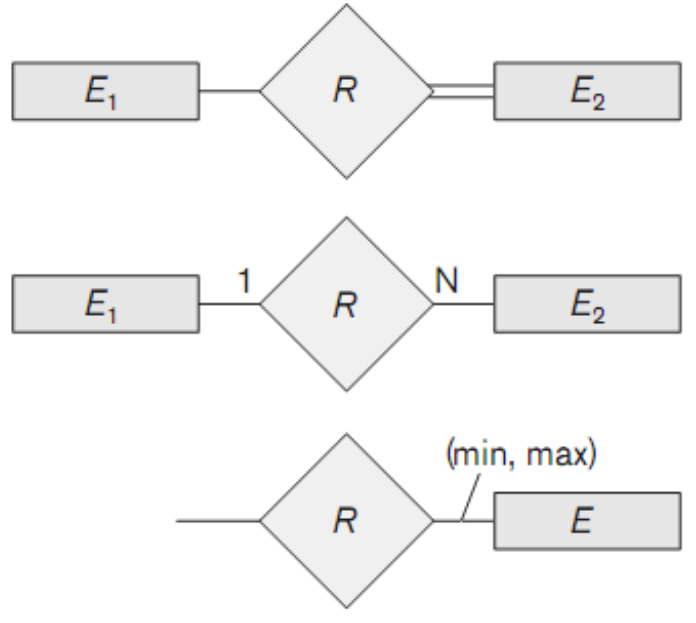
\includegraphics[width=0.45\textwidth]{images/erd/constraints.png}
        \caption{Structural Constraints on Relationship Types}
        \label{fig:structural-constraints}
    \end{figure}
\end{enumerate}





